% DRAFT (Phase 1b, 2026-11-19) -- NOT \input into main.tex yet.
% Insert into sections/07_discussion.tex (before "Threats to validity") once
% (1) the v3b full-corpus run is analysed and (2) the user has decided the primary
% protocol (v3 `fold` vs v2). Numbers: results/phase1b/whowhen.json;
% figure: figures/fig_whowhen.pdf (analysis_v3/phase1b.py). Exploratory, post hoc.

\subsection{Who or when? An exploratory decomposition}
\label{sec:whowhen}
This analysis was not planned; we report it as exploratory. A window-level score can be high because a model ranks \emph{students} (who is attentive) or because it follows attention \emph{over time} (when a student is attentive). We split the correlation between prediction and label into a between-person part (per-person means) and a within-person part (after removing them; Fig.~\ref{fig:whowhen}). On the DIPSER paper slice, 59\% of the label variance lies between the 20 persons, and every model follows that structure: the best single stream (face mesh, soft target) reaches between-person $r=0.41$ (v2 protocol) and $0.43$ (person-stratified folds with training-fold standardisation), but within-person $r$ of only $0.08$ and $0.03$. The best fusion behaves alike (between $0.22$/$0.36$, within $0.09$/$0.01$). Standardising features within each session, which removes between-student offsets, leaves every stream near chance (best QWK $0.075$). DAiSEE labels are much less person-level (12\% between persons) and its models are weak on both axes (within $r\le 0.05$). EngageNet (51\% between persons) is the one dataset where facial geometry and head pose also track changes within a person (within $r=0.19$), with between-person $r$ of $0.51$--$0.60$. On the paper slice, DIPSER models therefore mostly recognise who is attentive, not when.

This is partly a property of the slice. Across the full DIPSER release (57 persons, 483 sessions, 35{,}649 windows) only 13\% of the label variance lies between persons, 20\% between class sessions (group $\times$ experiment) and 49\% between student-sessions; labels of the other students in the same class session predict a window's label with QWK $0.37$ without any sensor input. On the full corpus (person-stratified folds, 3 seeds), every stream stays low (best: face mesh, QWK $0.116$, 95\% CI $[0.077, 0.158]$), within-session agreement is real but small ($r\le 0.05$), and no stream beats a control trained on a \emph{classmate's} labels at the same moment (QWK $\approx 0.08$): what the sensors capture is mostly shared by the class, not specific to the student. For classroom use the distinction matters: a trait-like score supports a profile of a student, a state-like score supports feedback during a lesson, and only the second is what attention \emph{recognition} usually promises.

% Figure environment to add with the paragraph:
% \begin{figure*}[t]
%   \centering
%   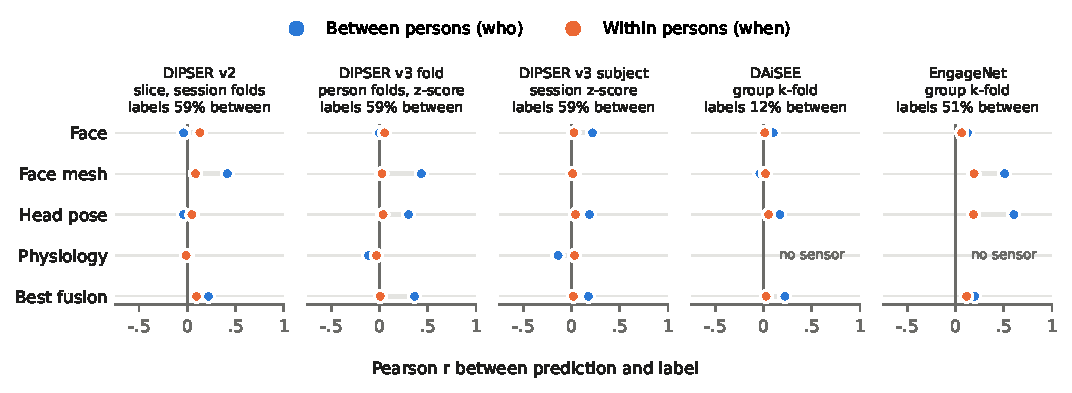
\includegraphics[width=\textwidth]{figures/fig_whowhen.pdf}
%   \caption{Between-person (who) and within-person (when) correlation of the best
%   configuration of each stream and the best fusion. Panel titles give the share of
%   label variance between persons. Exploratory, post hoc.}
%   \label{fig:whowhen}
% \end{figure*}
